\documentclass[11pt]{report}

\usepackage{fontspec}
\usepackage[margin=1.1in]{geometry}
\usepackage{booktabs}
\usepackage{tabularx}
\usepackage{longtable}
\usepackage{array}
\usepackage{ragged2e}
\usepackage{float}
\usepackage{graphicx}
\usepackage{xcolor}
\usepackage{amssymb}
\usepackage{titlesec}
\usepackage{setspace}
\usepackage{enumitem}
\usepackage[most]{tcolorbox}
\IfFileExists{microtype.sty}{\usepackage{microtype}}{}
\usepackage[hidelinks,bookmarks=true,bookmarksnumbered=true]{hyperref}

% --- Fonts (xelatex) ---
\setmainfont{DejaVu Serif}[
  Ligatures=TeX,
  Scale=0.96
]
\newfontfamily\headingfont{DejaVu Sans}[Scale=0.96]
\setmonofont{DejaVu Sans Mono}[Scale=0.86]

% --- Paragraph style: space between, no indent (modern look) ---
\usepackage{parskip}
\onehalfspacing
\setlength{\emergencystretch}{3em}

% --- Colours ---
\definecolor{diaaccent}{HTML}{2C3E66}
\definecolor{diarule}{HTML}{8896B8}
\definecolor{diaboxbg}{HTML}{F2F4F9}

% --- Heading style (clean, sans, accented) ---
\titleformat{\section}
  {\headingfont\Large\bfseries\color{diaaccent}}
  {\thesection}{0.7em}{}
\titleformat{\subsection}
  {\headingfont\large\bfseries\color{diaaccent}}
  {\thesubsection}{0.6em}{}
\titleformat{\subsubsection}
  {\headingfont\normalsize\bfseries\color{diaaccent}}
  {\thesubsubsection}{0.5em}{}
\titleformat{\paragraph}[runin]
  {\headingfont\normalsize\bfseries\color{diaaccent}}
  {}{0em}{}[.\quad]
\titlespacing*{\paragraph}{0pt}{0.6em}{0.5em}

% Chapter title styling for the appendix opener.
\titleformat{\chapter}[display]
  {\headingfont\huge\bfseries\color{diaaccent}}
  {\chaptertitlename\ \thechapter}{12pt}{\Huge}

% --- Blockquote box ---
\newtcolorbox{diabox}{
  colback=diaboxbg,
  colframe=diarule,
  boxrule=0.4pt,
  leftrule=3pt,
  arc=2pt,
  left=8pt, right=8pt, top=6pt, bottom=6pt,
  breakable
}

% Spacing for tables a touch more open.
\setlength{\tabcolsep}{5pt}

\hypersetup{
  pdftitle={Dramatistic-Involvement Analysis (DIA)},
  pdfauthor={DIA Method},
  pdfsubject={A Unified Method for Analyzing User Behavior in Video-Game Environments},
  colorlinks=false,
  linkcolor=diaaccent,
  urlcolor=diaaccent
}

\begin{document}


\begin{titlepage}
\centering
\vspace*{2.2cm}

{\headingfont\bfseries\color{diaaccent}\fontsize{30}{36}\selectfont
Dramatistic-Involvement Analysis (DIA)\par}

\vspace{1.0cm}
{\color{diarule}\rule{0.72\textwidth}{1pt}\par}
\vspace{1.0cm}

{\headingfont\Large
A Unified Method for Analyzing User Behavior\\[0.25em]
in Video-Game Environments\par}

\vspace{2.6cm}

{\large
Integrating Kenneth Burke's Dramatistic Pentad\\[0.35em]
(\textit{A Grammar of Motives} 1945 + \textit{A Rhetoric of Motives} 1950)\\[0.6em]
with Gordon Calleja's Player Involvement Model\\[0.35em]
(\textit{In-Game} 2011)\par}

\vfill

{\large\headingfont 2026-05-27\par}
\vspace{1.0cm}
\end{titlepage}

\hypersetup{linkcolor=diaaccent}
\renewcommand{\contentsname}{Contents}
\tableofcontents
\clearpage

\begin{tcolorbox}[
  colback=diaboxbg, colframe=diaaccent, boxrule=0.8pt, arc=3pt,
  left=10pt, right=10pt, top=8pt, bottom=8pt,
  title={\headingfont\bfseries Quick-Reference Card --- The 8 DIA Steps},
  coltitle=white, colbacktitle=diaaccent, fonttitle=\bfseries
]
\setlist[description]{leftmargin=6.6em, style=sameline, font=\bfseries\color{diaaccent}}
\begin{description}[itemsep=2pt, topsep=2pt]
  \item[Step 0] Scope \& circumference --- fix the episode boundary and representative anecdote.
  \item[Step 1] Involvement profile (Axis I) --- six PIM dimensions $\times$ macro/micro, with intensity \& trajectory.
  \item[Step 2] Motive grammar (Axis M) --- fill the six pentad terms; mark the featured term(s).
  \item[Step 3] Ratio dynamics --- name the dominant ratio (the motive-engine).
  \item[Step 4] Crosswalk binding --- fuse Axis M to Axis I via the validated crosswalk.
  \item[Step 5] Identification \& consubstantiation --- the keystone; test incorporation rubric R1--R5.
  \item[Step 6] Attitude --- competitive / completionist / explorer / devotional / ironic-meta; elation$\leftrightarrow$accidie.
  \item[Step 7] Diagnosis \& ends --- one-paragraph behavioral diagnosis $+$ the end it serves.
\end{description}
\end{tcolorbox}

\clearpage
% ==== source: game-behavior-analysis-method.md ====
\section{Dramatistic-Involvement Analysis (DIA)}

\subsection{A Unified Method for Analyzing User Behavior in Video-Game Environments}


\textbf{Integrating Kenneth Burke's dramatistic pentad (\textit{A Grammar of Motives} 1945 + \textit{A Rhetoric of Motives} 1950) with Gordon Calleja's Player Involvement Model (\textit{In-Game} 2011).}


\textbf{Version}: 1.0 · \textbf{Date}: 2026-05-27 · \textbf{Plan}: \texttt{plans/\discretionary{}{}{}burke-\discretionary{}{}{}calleja-\discretionary{}{}{}game-\discretionary{}{}{}behavior-\discretionary{}{}{}integration.\discretionary{}{}{}md} (Phase 3) \textbf{Inputs}: \texttt{validated-\discretionary{}{}{}crosswalk.\discretionary{}{}{}json} (Phase 2); \texttt{gm-\discretionary{}{}{}pentad-\discretionary{}{}{}operationalization-\discretionary{}{}{}manual.\discretionary{}{}{}md}; \texttt{ig-\discretionary{}{}{}pim-\discretionary{}{}{}operationalization-\discretionary{}{}{}manual.\discretionary{}{}{}md}; \texttt{rm-\discretionary{}{}{}identification-\discretionary{}{}{}consubstantiation-\discretionary{}{}{}manual.\discretionary{}{}{}md}; \texttt{rm-\discretionary{}{}{}attitude-\discretionary{}{}{}as-\discretionary{}{}{}sixth-\discretionary{}{}{}term.\discretionary{}{}{}md}.


\textbf{Provenance discipline.} Burke's and Calleja's own claims are reported as source material (\texttt{burke-\discretionary{}{}{}direct} / \texttt{calleja-\discretionary{}{}{}direct}). Every binding \textit{between} the two frameworks, and every application to game behavior, is \texttt{anticipatory-\discretionary{}{}{}projection} — a dissertation construction neither author makes. Part F (ontological grounding in the Actualization-of-Desire hierarchy) is a \textbf{deferred stub} per user direction.


\vspace{0.4em}\hrule\vspace{0.8em}


\subsection{Part A — Theoretical Integration: Why Two Axes}


\subsubsection{A.1 The gap each framework leaves}


\textbf{Calleja's PIM} answers \textit{what is the player doing, and how are they engaged?} It decomposes involvement into six dimensions — \textbf{kinesthetic, spatial, shared, narrative, affective, ludic} — each operating across a \textbf{macro} phase (off-line: planning, forums, anticipation) and a \textbf{micro} phase (in-session, moment-to-moment), culminating in \textbf{incorporation} (the player absorbed into, and absorbing, the gameworld). It is a phenomenology of engagement. What it does not supply is \textit{motive}: it can establish that a player is intensely ludically and kinesthetically involved without explaining why the behavior takes the shape it does or what the player is doing it \textit{for}.


\textbf{Burke's pentad} answers \textit{why — under what grammar of motive?} Any stretch of human action can be addressed through five terms — \textbf{Act} (what was done), \textbf{Scene} (where/in what situation), \textbf{Agent} (who), \textbf{Agency} (by what means), \textbf{Purpose} (to what end) — plus the later sixth term \textbf{Attitude} (in what disposition), and, decisively, through the \textbf{ratios} between them (how Scene constrains Act, how Act remakes Agent, and so on). It is a grammar of motives. What it does not supply is the \textit{structural texture} of engagement through which a motive is actually lived in a game — the phase-distinction, the dimensional intensities, the internalization trajectories that Calleja makes visible.


\subsubsection{A.2 The fused unit of analysis}


DIA treats these as \textbf{two axes of a single apparatus}:


\begin{itemize}
\item \textbf{Axis M (Motive — Burke):} the six terms + the ratios (the \textit{dynamics}) + identification/consubstantiation (the \textit{bond}).
\item \textbf{Axis I (Involvement — Calleja):} the six dimensions $\times$\allowbreak  macro/micro phase.
\end{itemize}


The \textbf{atomic unit of a DIA analysis is the grid cell} \texttt{(motive term × involvement dimension × phase)} — e.g. \textit{(Agency $\times$\allowbreak  Kinesthetic $\times$\allowbreak  micro)} = "the player's moment-to-moment use of the control scheme as the \textit{means} of action." The \textbf{ratios} describe motion \textit{between} cells. The \textbf{keystone} — consubstantiation/incorporation — is read \textit{across} the whole grid: it is simultaneously the motive-grammar endpoint (Burke's \textit{ultimate identification}) and the involvement endpoint (Calleja's \textit{incorporation}).


This is not two reports stapled together. A single behavioral phenomenon is read \textit{once}, through a grid whose rows and columns are each other's explanations: the motive term tells you why the dimensional involvement has the character it does, and the dimensional involvement tells you how the motive is concretely enacted.


\subsubsection{A.3 What each axis adds to the other}


\begin{table}[H]
\renewcommand{\arraystretch}{1.25}
\begin{tabularx}{\textwidth}{>{\RaggedRight\arraybackslash}X>{\RaggedRight\arraybackslash}X}
\toprule
Axis M (Burke) adds to Calleja & Axis I (Calleja) adds to Burke \\
\midrule
\textbf{Motive} behind dimensional intensity (why this involvement, toward what) & \textbf{Phase distinction} (macro/micro) the pentad lacks \\
\textbf{Cross-dimensional ratios} (PIM treats dimensions as independent; ratios are inherently multi-dimensional) & \textbf{Dimensional granularity + intensity + internalization trajectory} \\
\textbf{Identification/consubstantiation} as the motive-mechanism beneath incorporation & \textbf{A grounded, interview-validated phenomenology} of the lived state the pentad only schematizes \\
\textbf{Attitude} as the disposition coloring any act & \textbf{Empirical method} (grounded-theoretic, in-environment interview) for evidencing claims \\
\bottomrule
\end{tabularx}
\end{table}


\subsubsection{A.4 The conflict the method must hold (not collapse)}


Burke is \textbf{grammatical-motivational} — action explained by motives located in pentad ratios; Calleja is \textbf{phenomenological-experiential} — action explained by player-reported lived states. The integration must treat Burke's motive-attribution as a \textit{theoretical supplement} to, not a \textit{displacement} of, Calleja's experiential primacy. Where the registers pull apart (e.g. Calleja's metaphor-disclaimer about incorporation vs. Burke's substance-realism), DIA \textbf{moves between registers as the analytic question requires} and marks which register is doing the work. The keystone bridge is a \textbf{homology, not an equation} (five divergences; see Part B.4). The method's discipline is to keep the two voices distinguishable on the page.


\vspace{0.4em}\hrule\vspace{0.8em}


\subsection{Part B — The Unified Grid}


\subsubsection{B.1 The validated crosswalk (the grid's spine)}


From \texttt{validated-\discretionary{}{}{}crosswalk.\discretionary{}{}{}json} (Phase 2; bindings confirmed bidirectionally against both texts):


\begin{table}[H]
\small
\renewcommand{\arraystretch}{1.25}
\begin{tabularx}{\textwidth}{>{\RaggedRight\arraybackslash}X>{\RaggedRight\arraybackslash}X>{\RaggedRight\arraybackslash}X>{\RaggedRight\arraybackslash}X}
\toprule
Motive term (Burke) & Primary involvement dim(s) (Calleja) & Secondary & Status \\
\midrule
\textbf{Act} & Ludic (the \textit{choosing}), Narrative & Kinesthetic (execution pole) & validated \\
\textbf{Scene} & Spatial & Kinesthetic (body-orientation) & validated — strongest \\
\textbf{Agent} & Shared & — & validated (deepened by consubstantiation) \\
\textbf{Agency} & Kinesthetic, Ludic (the \textit{rule-system}) & — & validated \\
\textbf{Purpose} & Ludic, Narrative & Affective (mastery/regulation) & validated \\
\textbf{Attitude} & Affective & \textit{(transverse — modifies all five above)} & validated + extended \\
\bottomrule
\end{tabularx}
\end{table}


\textbf{The four-binding bijective core} — \texttt{Scene↔Spatial}, \texttt{Agent↔Shared}, \texttt{Agency↔Kinesthetic}, \texttt{Attitude↔Affective} — was reached \textit{independently} from both directions and is the grid's load-bearing structure.


\textbf{The Ludic split} (the one productive divergence): the \textbf{rule-system} (mechanics, cooldowns, economy) is \textbf{Agency} (means); the \textbf{act of choosing-under-repercussion} is \textbf{Act + Purpose}. One Calleja dimension is dramatistically two moments; the method reads them as separate cells.


\subsubsection{B.2 The ratios — the dynamics layer}


Cells are static placements; \textbf{ratios are the engine.} The ratios most diagnostic of game behavior (Burke's gloss $\rightarrow$\allowbreak  the game-behavior question DIA asks):


\begin{table}[H]
\renewcommand{\arraystretch}{1.25}
\begin{tabularx}{\textwidth}{>{\RaggedRight\arraybackslash}X>{\RaggedRight\arraybackslash}X>{\RaggedRight\arraybackslash}X}
\toprule
Ratio & Game-behavior question & Bound dimension-pair \\
\midrule
\textbf{Scene–Act} & How does the gameworld constrain/enable what the player does? & Spatial $\times$\allowbreak  Ludic/Narrative \\
\textbf{Act–Agent} & How does what the player does remake who they are (alterbiography)? & Ludic/Narrative $\times$\allowbreak  Shared \\
\textbf{Agency–Purpose} & How do available means shape — or \textit{become} — the player's ends? & Kinesthetic/rule-system $\times$\allowbreak  Ludic-goal \\
\textbf{Scene–Agent} & How does the gameworld/social-rank qualify the inhabiting player? & Spatial/Shared \\
\textbf{Agent–Agent} (co/counter) & How do co-agents and counter-agents structure motive? & Shared (cohabitation/cooperation/competition) \\
\bottomrule
\end{tabularx}
\end{table}


The \textbf{Agency–Purpose} ratio is the single most diagnostic for compulsion: when means drift into becoming their own ends (the grind, the speedrun, the daily-login), Burke's "means become end" \textit{is} the behavioral signature Calleja's ludic-intensity-without-stated-goal records.


\subsubsection{B.3 Attitude — the transverse modifier}


Attitude is not a sixth column; it is the \textit{disposition-with-which} any cell is enacted. The five player-attitude registers (from \texttt{rm-\discretionary{}{}{}attitude-\discretionary{}{}{}as-\discretionary{}{}{}sixth-\discretionary{}{}{}term} §E), each foregrounding \textbf{Affective} involvement:


\textbf{Competitive} (agonistic striving up the rank-hierarchy) · \textbf{Completionist} (engagement sustained by the impossibility of final acquisition — the suspended act) · \textbf{Explorer} (dwelling-toward and ascending-through the scene) · \textbf{Devotional} (reverent self-subordination to the gameworld's order — toward incorporation at its fullest) · \textbf{Ironic-meta} (detached, playing \textit{with} the game's rhetoric — speedrun, meta-gaming).


A player oscillates among registers; any act can be performed in more than one. The register is the affective-dispositional coding of the whole grid for that episode.


\subsubsection{B.4 The keystone — Consubstantiation $\leftrightarrow$\allowbreak  Incorporation (read across the grid)}


The vertical binding that the whole method turns on (\texttt{rm-\discretionary{}{}{}identification-\discretionary{}{}{}consubstantiation-\discretionary{}{}{}manual} §D):


\begin{itemize}
\item Burke's \textbf{consubstantiation} — to identify A with B is to make them "substantially one … yet a distinct locus of motives — both joined and separate" (RM-01 p.21), grounded in \textit{acting-together}.
\item Calleja's \textbf{incorporation} — assimilation axis (world $\rightarrow$\allowbreak  consciousness) + embodiment axis (player $\rightarrow$\allowbreak  world via avatar) + simultaneity condition (IG-10 p.169).
\item \textbf{Homology:} "substantially one" $\rightarrow$\allowbreak  assimilation; "distinct locus / the avatar" $\rightarrow$\allowbreak  embodiment; "both-joined-and-separate" $\rightarrow$\allowbreak  simultaneity; \textit{acting-together} $\rightarrow$\allowbreak  the spatial+kinesthetic cornerstone. \textbf{Ultimate identification} (mystic dissolution into boundless being, RM-07 p.333) $\rightarrow$\allowbreak  incorporation at its fullest.
\item \textbf{Five divergences keep it a homology, not an equation:} medium (symbolic vs phenomenological), ontological status (real-or-persuaded vs experiential), grounding theory (substance-metaphysics vs experientialist cognition), directionality (asymmetric-deployed vs bidirectional), scope (society-wide+self-address vs ergodic-bounded).
\end{itemize}


When a DIA analysis finds the player \textit{substantially one with} avatar/guild/world while remaining a distinct locus of motives, it is reading consubstantiation and incorporation as the same event from two sides.


\vspace{0.4em}\hrule\vspace{0.8em}


\subsection{Part C — The Method (step-by-step)}


\textbf{DIA is a runnable protocol.} Inputs: a documented player episode — a play recording or detailed trace; observation notes; (ideally) a think-aloud or post-session semi-structured interview (Calleja's grounded-theoretic standard); and, for the macro phase, the player's off-line traces (forum/Discord posts, theorycrafting, guild activity). Output: a structured \textbf{DIA report} + a \textbf{filled grid} + a \textbf{one-paragraph behavioral diagnosis}.


\subsubsection{Step 0 — Scope \& circumference}

Fix the episode boundary and the \textit{representative anecdote} (Burke) / \textit{unit of analysis} (Calleja): is the object a single session, a specific incident (a raid wipe, a betrayal, a first clear), a whole character-career, or a player's relationship to the game over months? Set the \textbf{circumference} deliberately — too wide and motive blurs; too narrow and the macro phase vanishes. State it explicitly.


\subsubsection{Step 1 — Involvement profile (Axis I)}

Map all six PIM dimensions $\times$\allowbreak  macro/micro. For each present dimension, note \textbf{intensity} (low/med/high), \textbf{internalization trajectory} (conceptual$\rightarrow$\allowbreak inhabited; conscious$\rightarrow$\allowbreak fluent; scripted$\rightarrow$\allowbreak alterbiographic), and \textbf{evidence} (which observation/interview datum supports it). Use Calleja's boundary criteria (e.g. inhabitation-criterion for Spatial; the symbolic/mimetic/symbiotic continuum for Kinesthetic). \textit{This is the "what is the player doing, structurally" pass.}


\subsubsection{Step 2 — Motive grammar (Axis M)}

Fill the six pentad terms for the episode — Act / Scene / Agent / Agency / Purpose / Attitude — recording what concretely occupies each (note that any term may have several fillers, and that Agent may \textit{shift} between player-as-self, avatar, and character). Identify the \textbf{featured term(s)}: which term is the locus of motive this episode foregrounds (e.g. an exploration session features Scene; a ranked match features Agency+Purpose). \textit{This is the "why — under what grammar" pass.}


\subsubsection{Step 3 — Ratio dynamics}

Identify the operative ratios (Part B.2) and name the \textbf{dominant} one. Ask what the player \textit{attributes their behavior to} — the situation (scene-act), their own development (act-agent), the tools (agency-purpose), the other players (agent-agent). The dominant ratio is the episode's motive-engine.


\subsubsection{Step 4 — Crosswalk binding (the fusion)}

Bind Axis M to Axis I using \texttt{validated-\discretionary{}{}{}crosswalk.\discretionary{}{}{}json}. For each featured motive term, read it through its bound dimension(s); for each high-intensity dimension, read it through its bound motive term. The fusion produces statements no single framework yields, e.g.: \textit{"the high ludic-micro intensity (I) is an Agency-Purpose collapse (M): the rule-system's means have become the player's ends."} Apply the \textbf{Ludic split} explicitly: is the ludic involvement about the \textit{rule-system} (Agency) or the \textit{choosing} (Act+Purpose)?


\subsubsection{Step 5 — Identification \& consubstantiation (the keystone)}

Analyze the player's nested identifications — with \textbf{avatar/character} (embodiment), \textbf{guild/faction/playerbase} (acting-together, "'Belonging' is rhetorical"). Locate where \textbf{consubstantiation} occurs (the player substantially one with X while remaining a distinct locus) and assess \textbf{incorporation} against the rubric (R1 assimilation, R2 embodiment, R3 simultaneity, R4 spatial+kinesthetic cornerstone, R5 blending). Note any \textbf{mystery / hierarchy / courtship} dynamics structuring the social field (Shared), and any \textbf{victimage / the kill} (scapegoating, toxicity) discharging hierarchic guilt.


\subsubsection{Step 6 — Attitude (the disposition)}

Identify the player's dominant attitude register(s) — competitive / completionist / explorer / devotional / ironic-meta (Part B.3) — and the \textbf{elation$\leftrightarrow$\allowbreak accidie} arc (sustained engagement vs. post-flow-break disengagement). Attitude is the affective-dispositional coloring of the whole grid; it is also an \textit{incipient act of identification} (the hinge to Step 5).


\subsubsection{Step 7 — Diagnosis \& ends}

Synthesize Steps 1–6 into a \textbf{one-paragraph behavioral diagnosis} that names: the featured motive term(s), the dominant ratio, the keystone state (mere-involvement vs incorporation; consubstantial vs strategic belonging), the attitude register, and the resulting behavior. Then apply it to the \textbf{end} the analysis serves (Part E).


\begin{diabox}
\textbf{Output template — the filled grid.} A 6$\times$\allowbreak 6 table (motive terms $\times$\allowbreak  dimensions) with the active cells marked and annotated, plus: featured-term(s), dominant-ratio, keystone-verdict, attitude-register, and the one-paragraph diagnosis. See the worked example (\texttt{worked-\discretionary{}{}{}example-\discretionary{}{}{}wow.\discretionary{}{}{}md}) for a completed instance.

\end{diabox}


\vspace{0.4em}\hrule\vspace{0.8em}


\subsection{Part D — Analytic-Question Battery}


Reorganized by the unified grid (merges and de-duplicates Burke \texttt{gm} §D and Calleja \texttt{ig} §D, plus integration questions). Ask only those relevant to the episode's featured terms.


\textbf{Scene / Spatial}

\begin{enumerate}
\item What features of the gameworld foreground themselves as the \textit{containing} condition of the player's acts? (Scene-Act)
\item Is space encountered as navigable inhabited place or as conceptual map? Can the player meaningfully get lost?
\item What does the player's \textit{physical room} contribute as outer Scene (couch vs. arcade vs. tournament stage)?
\end{enumerate}


\textbf{Act / Ludic(choosing) + Narrative}

\begin{enumerate}
\item What is the session-arc act, and what sub-acts compose it (microtactic $\rightarrow$\allowbreak  tactic $\rightarrow$\allowbreak  strategy)?
\item Where does \textit{act} collapse into mere \textit{motion} (sheer grinding, autopilot)? (Burke's act-motion watershed)
\item How does scripted narrative interweave with the player's alterbiography? Which dominates?
\end{enumerate}


\textbf{Agent / Shared}

\begin{enumerate}
\item Who is acting — the player-as-self, the avatar, the character? When does the agent-position \textit{shift}?
\item Who are the co-agents (guild, party) and counter-agents (PvP opponents, AI, the designer-as-counter-agent)?
\item Where do super-agents emerge (the guild, the server, the community, the studio)?
\end{enumerate}


\textbf{Agency / Kinesthetic + Ludic(rule-system)}

\begin{enumerate}
\item What means is the player wielding — controller (Kinesthetic), rule-system (Ludic), other players' moves, third-party tools?
\item Where does the control scheme become transparent (fluent) vs. announce itself (friction)?
\item \textit{Ludic split:} is a given ludic behavior about operating the rule-\textit{system} (Agency) or about \textit{choosing-under-repercussion} (Act+Purpose)?
\end{enumerate}


\textbf{Purpose / Ludic-goal + Narrative}

\begin{enumerate}
\item Game-internal goal? Flow-seeking? Affective regulation? Social status? Mastery? Exploration? Narrative resolution? External (streaming/esports)?
\item \textbf{(Agency–Purpose, the compulsion diagnostic)} Where do means become ends — the grind, daily-login, speedrun, min-max — as a purpose-drift?
\item What is the ultimate term / "god-term" (RM-05) that ranks all the player's other goals (the win-condition, the prestige currency, the meta apex)?
\end{enumerate}


\textbf{Attitude / Affective (transverse)}

\begin{enumerate}
\item In what disposition is the player acting — competitive / completionist / explorer / devotional / ironic-meta?
\item Where is the episode on the elation$\leftrightarrow$\allowbreak accidie arc (sustained flow vs. post-break disengagement)?
\item What is the player's attitude \textit{toward the game's rhetoric} — playing within it, or with it (meta/irony)?
\end{enumerate}


\textbf{Keystone / Identification, consubstantiation, incorporation}

\begin{enumerate}
\item With whom/what is the player made substantially one (avatar, guild, faction, world) — and where do they remain a distinct locus of motives?
\item Does the episode meet the incorporation rubric (R1–R5), or is it mere-involvement? Which component fails if not?
\item Is belonging \textit{consubstantial} (genuine acting-together) or \textit{strategic/persuaded} (cunning identification, "by default")? (RM-01 tension T1)
\item \textbf{(Social hierarchy)} Where do mystery, hierarchy, and courtship structure the Shared field (elite allure, guild initiation/hazing, rank deference)?
\item \textbf{(Victimage)} Does hierarchic guilt discharge in a scapegoat (toxicity, blaming, out-group hostility)?
\end{enumerate}


\textbf{Cross-cutting}

\begin{enumerate}
\item Which single grid region (term $\times$\allowbreak  dimension) carries the episode's behavioral weight — and what would change if it were absent?
\item Which register (Burke-motivational vs Calleja-experiential) better explains a contested datum, and why?
\end{enumerate}


\vspace{0.4em}\hrule\vspace{0.8em}


\subsection{Part E — Ends: What the Method Is For}


DIA earns its complexity by yielding diagnoses neither framework produces alone. Four primary ends:


\subsubsection{E.1 Game-design critique}

Diagnose \textbf{compulsion loops and dark patterns} structurally rather than moralistically: a daily-login or gacha loop is an \textbf{Agency–Purpose collapse} (means engineered to become ends) operating on \textbf{Ludic} involvement, often sustained by \textbf{hierarchy/mystery} (FOMO, opaque rates) on the \textbf{Shared/Affective} dimensions. The method names \textit{which} motive-mechanism a design exploits and \textit{which} involvement dimension carries it — actionable for ethical design review.


\subsubsection{E.2 Player-experience research}

The filled grid is a \textbf{coding instrument} for qualitative play research, parallel to and extending Calleja's grounded-theoretic scheme: it codes not only \textit{what} dimensions are involved but \textit{what motive} and \textit{what disposition} animate them, with both-sides evidentiary anchoring.


\subsubsection{E.3 Social \& identity behavior}

Explain \textbf{guild attachment, toxicity, and betrayal} via the keystone + social-motive apparatus: attachment is \textbf{consubstantiation} through acting-together; toxicity is \textbf{victimage} discharging \textbf{hierarchic} guilt; a guild-betrayal (e.g. the EVE \textit{Guiding Hand} heist) is a \textbf{consubstantiation-rupture} — the betrayer exploited a Shared-dimension identification that was real enough to be weaponized. DIA gives these a vocabulary beyond "engagement."


\subsubsection{E.4 Comparative game analysis}

Different games \textbf{foreground different grid regions}: a walking simulator lives in Scene$\times$\allowbreak Spatial + Attitude(explorer); a fighting game in Agency$\times$\allowbreak Kinesthetic + Act; an MMO raid in Agent$\times$\allowbreak Shared + the keystone. Mapping a game's \textit{characteristic grid region} is a compact comparative signature.


\vspace{0.4em}\hrule\vspace{0.8em}


\subsection{Part F — Ontological Grounding \textit{(DEFERRED — STUB)}}


\textbf{Per user direction (2026-05-27), this layer is reserved, not built.} When the Actualization-of-Desire hierarchy (A$_0$ sensible object $\rightarrow$\allowbreak  A$_1$ perception $\rightarrow$\allowbreak  A$_2$ \textit{phantasma} $\rightarrow$\allowbreak  A$_3$ noetic/doxastic/mnemonic/anticipatory $\rightarrow$\allowbreak  A$_4$ completed action) is finalized, a future pass will populate the per-term ontological targets below and situate the whole DIA grid within that chain. \textbf{No content is generated now.}


\begin{table}[H]
\renewcommand{\arraystretch}{1.25}
\begin{tabularx}{\textwidth}{>{\RaggedRight\arraybackslash}X>{\RaggedRight\arraybackslash}X>{\RaggedRight\arraybackslash}X}
\toprule
Motive term & Ontological-grounding slot (Aristotle/Heidegger) & Status \\
\midrule
Act & \textit{energeia} / \textit{dynamis} (Burke's own Aristotle/Aquinas exegesis, GM-06) — EXEGETICAL anchor & reserved \\
Scene & \textit{In-der-Welt-sein} / \textit{Befindlichkeit} — or Uexküll \textit{Umwelt} (candidate, more apt for bounded designed worlds) & reserved \\
Agent & \textit{psuchē} / \textit{Dasein} / \textit{Mitsein} & reserved \\
Agency & \textit{technē} / \textit{organon} & reserved \\
Purpose & \textit{telos} / \textit{Worumwillen} & reserved \\
Attitude & \textit{hexis} / disposition; the incipient act between \textit{dynamis} and \textit{energeia} & reserved \\
Keystone (consubstantiation/incorporation) & the A$_3$$\rightarrow$\allowbreak A$_4$ completion; the actualization of desire as substantial union & reserved — the likely primary integration site \\
\bottomrule
\end{tabularx}
\end{table}


\textit{Hook note:} the keystone (consubstantiation$\leftrightarrow$\allowbreak incorporation as substantial union completing a motion) is the natural attachment point to the A$_3$$\rightarrow$\allowbreak A$_4$ segment of the chain; this is where the future ontological pass should begin.


\vspace{0.4em}\hrule\vspace{0.8em}


\subsection{Appendix — One-line summary}


\textbf{DIA reads a player episode once, through a grid whose rows are Burke's six motive terms and whose columns are Calleja's six involvement dimensions, bound by a bidirectionally-validated crosswalk, driven by Burke's ratios, and anchored by the consubstantiation$\leftrightarrow$\allowbreak incorporation keystone — to produce a behavioral diagnosis that says not just \textit{what} the player is doing and \textit{how} engaged they are, but \textit{why} and \textit{in what disposition}.}


\textit{Content-filter: PASS — all Burke/Calleja prose paraphrased, no $\geq$25-word verbatim. Cross-framework bindings and game-behavior claims are \texttt{anticipatory-\discretionary{}{}{}projection}.}


\clearpage
% ==== source: worked-example-wow.md ====
\section{Worked Example — Dramatistic-Involvement Analysis of a \textit{World of Warcraft} Raid-Progression Night}


\textbf{Method}: \texttt{game-\discretionary{}{}{}behavior-\discretionary{}{}{}analysis-\discretionary{}{}{}method.\discretionary{}{}{}md} (DIA, Parts C steps 0–7) · \textbf{Crosswalk}: \texttt{validated-\discretionary{}{}{}crosswalk.\discretionary{}{}{}json} \textbf{Date}: 2026-05-27 · \textbf{Plan}: \texttt{plans/\discretionary{}{}{}burke-\discretionary{}{}{}calleja-\discretionary{}{}{}game-\discretionary{}{}{}behavior-\discretionary{}{}{}integration.\discretionary{}{}{}md} (Phase 4)


\begin{diabox}
\textbf{On the example's status.} This is a \textit{representative anecdote} (Burke's term) — a composite progression-raid night synthesized from well-documented \textit{WoW} raiding culture (25-player roster, DKP/loot-council economies, voice comms, boss-mods, combat-log parses, attendance pressure, post-progression burnout) and from Calleja's own grounded-theoretic \textit{WoW} interview dispositions (Rheric, Kumacho, Muun, Baal; the Sara Andrews server-governance case). It is illustrative, not a claim about any specific named individual. \textit{WoW} is chosen because Calleja analyzed it directly (IG-APX; manual §C), so the involvement axis is already empirically grounded — isolating what DIA \textit{adds}. All cross-framework and game-behavior claims are \texttt{anticipatory-\discretionary{}{}{}projection}.

\end{diabox}


\vspace{0.4em}\hrule\vspace{0.8em}


\subsection{The episode (raw description)}


A 25-player guild, three weeks into progression on an end-boss, raids 19:30–23:00 on a weeknight. The night is \textasciitilde{}18 attempts ("pulls"), each ending in a wipe at progressively later boss phases, until pull 17 — a clean execution that drops the boss with two players left alive. Euphoria on voice comms; a screenshot of the corpse; loot is distributed by loot council; one long-attending DPS player is passed over for the trinket and goes quiet. Afterward, half the raid lingers in voice for an hour replaying the kill; two players log off immediately to post the parse. Over the following week, attendance softens — the characteristic post-progression trough.


\vspace{0.4em}\hrule\vspace{0.8em}


\subsection{Step 0 — Scope \& circumference}


\textbf{Unit of analysis:} the single progression night (19:30–23:00), with a macro-phase penumbra of the surrounding week (theorycrafting before, attendance-softening after). \textbf{Representative anecdote:} the wipe$\rightarrow$\allowbreak wipe$\rightarrow$\allowbreak first-kill arc is the representative form of \textit{WoW} end-game raiding; the loot-council passing-over is the representative form of its hierarchic-guilt structure. Circumference set deliberately at "one night + its week-long penumbra" so both micro (the pulls) and macro (scheduling, parse-posting, burnout) are in frame.


\vspace{0.4em}\hrule\vspace{0.8em}


\subsection{Step 1 — Involvement profile (Axis I)}


\begin{table}[H]
\small
\renewcommand{\arraystretch}{1.25}
\begin{tabularx}{\textwidth}{>{\RaggedRight\arraybackslash}X>{\RaggedRight\arraybackslash}X>{\RaggedRight\arraybackslash}X>{\RaggedRight\arraybackslash}X>{\RaggedRight\arraybackslash}X}
\toprule
Dimension & Intensity & Macro phase & Micro phase & Internalization trajectory \\
\midrule
\textbf{Kinesthetic} & High & between-pull rotation rehearsal & class-rotation + reaction to boss mechanics & conscious$\rightarrow$\allowbreak fluent (veterans fluent; one undergeared recruit still conscious) \\
\textbf{Spatial} & Med–High & encounter-arena memorized between sessions & foot-positioning, boss-room hazard zones & conceptual$\rightarrow$\allowbreak inhabited (the arena is "known ground" by pull 10) \\
\textbf{Shared} & \textbf{Very high} & roster/attendance, Discord theorycraft, loot politics & 25-way voice coordination, role interdependence & cohabitation$\rightarrow$\allowbreak cooperation$\rightarrow$\allowbreak (competition for loot) \\
\textbf{Narrative} & Med & speculation about post-kill content & thin scripted lore; \textbf{heavy alterbiography} ("the night we finally got it") & scripted$\rightarrow$\allowbreak alterbiographic (the kill becomes a story they will retell) \\
\textbf{Affective} & \textbf{Very high} & anticipatory dread/excitement & wipe-frustration $\rightarrow$\allowbreak  kill-euphoria; the passed-over player's deflation & rising tension across pulls; discharge at the kill \\
\textbf{Ludic} & \textbf{Very high} & DKP/loot planning, strategy revision & per-pull plan$\rightarrow$\allowbreak execute$\rightarrow$\allowbreak wipe$\rightarrow$\allowbreak re-plan loop & strategy$\rightarrow$\allowbreak tactics$\rightarrow$\allowbreak microtactics fully operative \\
\bottomrule
\end{tabularx}
\end{table}


\textit{Reading:} all six dimensions present and blended; Shared, Affective, and Ludic are the load-bearing dimensions; Kinesthetic and Spatial are internalized (cornerstone met) for the veterans. This is, on Calleja's own terms, a strong \textbf{incorporation} candidate (R4 cornerstone met, R5 blending high) — Step 5 tests it.


\vspace{0.4em}\hrule\vspace{0.8em}


\subsection{Step 2 — Motive grammar (Axis M)}


\begin{table}[H]
\renewcommand{\arraystretch}{1.25}
\begin{tabularx}{\textwidth}{>{\RaggedRight\arraybackslash}X>{\RaggedRight\arraybackslash}X>{\RaggedRight\arraybackslash}X}
\toprule
Term & Filler(s) this episode & Featured? \\
\midrule
\textbf{Act} & the \textit{progression kill} (composed of 17 sub-act "pulls"); each pull = plan$\rightarrow$\allowbreak execute$\rightarrow$\allowbreak wipe & featured \\
\textbf{Scene} & the boss arena; the raid roster as a social scene; the weeknight time-box; the guild's competitive standing on the server & — \\
\textbf{Agent} & \textbf{shifting}: the individual player $\leftrightarrow$\allowbreak  the player's avatar/role (tank/healer/DPS) $\leftrightarrow$\allowbreak  the \textbf{raid-as-collective-agent} ("we got it") & featured (the shift is the story) \\
\textbf{Agency} & the rule-system (boss mechanics, cooldowns, DKP), the controls, voice comms, boss-mods/parses as instruments & — \\
\textbf{Purpose} & the \textbf{god-term}: the \textit{first kill} (guild progression), subordinating loot, parses, fun; secondary: loot acquisition; mastery; belonging & featured \\
\textbf{Attitude} & dominant \textbf{competitive}, shading \textbf{devotional} at the kill; the passed-over player slides toward \textbf{accidie} & featured \\
\bottomrule
\end{tabularx}
\end{table}


\textbf{Featured terms:} Act (the kill), Agent (the self$\leftrightarrow$\allowbreak collective shift), Purpose (the progression god-term), modulated by a competitive$\rightarrow$\allowbreak devotional Attitude. The episode's motive is \textit{the collective actualization of a difficult act under a subordinating purpose.}


\vspace{0.4em}\hrule\vspace{0.8em}


\subsection{Step 3 — Ratio dynamics}


\begin{itemize}
\item \textbf{Agency–Purpose (dominant):} the rule-system's means (rotations, cooldown-stacking, positioning) are bent wholly toward the single purpose of the kill; for the night, \textit{means are subordinated to end} — the healthy inverse of compulsion's "means become end." But note the macro risk: once the god-term (first kill) is consumed, the means lose their ordering purpose $\rightarrow$\allowbreak  the \textbf{attendance trough} (Step 7).
\item \textbf{Act–Agent:} the kill \textit{remakes the agents} — "we are now a guild that has killed this boss" (alterbiography; the collective-agent is constituted by the act). This is the night's identity-payoff.
\item \textbf{Scene–Act:} the boss arena and the 25-role interdependence \textit{constrain and enable} the act — the encounter's design dictates the shape of legitimate play (rails the raid onto a narrow solution path).
\item \textbf{Agent–Agent (co/counter):} the raid is a \textbf{collective agent} against the boss as \textbf{counter-agent}; internally, the loot economy introduces a competitive agent-agent ratio (the passed-over player vs. the loot recipient).
\end{itemize}


\textbf{Player attribution:} the raid attributes success to \textit{coordination} (Act-Agent: "we pulled it together") and difficulty to \textit{the encounter} (Scene-Act: "the design is punishing") — a healthy externalization that protects individual agents from blame, until the loot decision relocates motive to \textit{agent-agent} rivalry.


\vspace{0.4em}\hrule\vspace{0.8em}


\subsection{Step 4 — Crosswalk binding (the fusion)}


Reading Axis M through Axis I via \texttt{validated-\discretionary{}{}{}crosswalk.\discretionary{}{}{}json}:


\begin{itemize}
\item \textbf{Purpose $\times$\allowbreak  Ludic + Narrative} $\rightarrow$\allowbreak  the progression god-term \textit{is} the very-high Ludic intensity: the plan$\rightarrow$\allowbreak execute$\rightarrow$\allowbreak wipe$\rightarrow$\allowbreak re-plan loop is Purpose enacted through Ludic involvement; the "night we got it" is Purpose closing into Narrative (alterbiography).
\item \textbf{Agent $\times$\allowbreak  Shared} $\rightarrow$\allowbreak  the agent-position shift (self$\rightarrow$\allowbreak collective) \textit{is} the very-high Shared involvement: 25-way cooperation is the dramatistic collective-agent being assembled in real time.
\item \textbf{Agency-split} $\rightarrow$\allowbreak  the Ludic split is visible: the \textbf{rule-system} (boss mechanics, DKP) operates as \textbf{Agency} (the means/instrument), while the \textbf{per-pull choosing-under-repercussion} is \textbf{Act+Purpose}. The DKP economy is pure Agency (an instrument for distributing a scarce good) — which is exactly why, when it produces the passing-over, it generates an \textit{Agency-level} grievance that the player experiences \textit{Affectively}.
\item \textbf{Attitude $\times$\allowbreak  Affective} $\rightarrow$\allowbreak  the competitive$\rightarrow$\allowbreak devotional arc \textit{is} the affective trajectory (rising tension $\rightarrow$\allowbreak  kill-euphoria); the passed-over player's competitive attitude, denied its loot-payoff, slides to \textbf{accidie} (post-flow-break deflation).
\end{itemize}


\textbf{Fusion statement (what neither framework says alone):} \textit{The night's behavior is a collective Act under a subordinating Purpose (god-term: the first kill), enacted through very-high Ludic + Shared involvement, in which the rule-system-as-Agency (DKP) — normally invisible — becomes affectively salient at the moment it allocates scarce reward against a long-attending agent, converting a cooperative agent-agent ratio into a competitive one and seeding the post-progression social trough.}


\vspace{0.4em}\hrule\vspace{0.8em}


\subsection{Step 5 — Identification \& consubstantiation (the keystone)}


\begin{itemize}
\item \textbf{Avatar/role identification:} each player is \textit{substantially one} with their role (tank/healer/DPS) — the role is the systemically-upheld locus through which they act in the raid — while remaining a distinct locus of motives (their own parse, their own loot interest). Classic consubstantiation: joined-and-separate.
\item \textbf{Guild/collective identification:} at the kill, the raid achieves \textbf{consubstantiation as collective agent} — "\textit{we} got it" is not a figure of speech but the lived state of acting-together (Burke's ground of consubstantiality, RM-01 p.21). The hour of lingering in voice afterward is the \textit{enacted-ritual} register (RM-07 Rattlesnake Club): consubstantiality through a shared solemn experience, the kill being the occasion, not the essence.
\item \textbf{Incorporation verdict (rubric R1–R5):} for the veteran raiders during the successful pull, \textbf{incorporation is MET} — R1 (the arena absorbed into consciousness), R2 (avatar-embodiment in the role), R3 (simultaneity during the clean execution), R4 (spatial+kinesthetic cornerstone met), R5 (4–5 dimensions blended). The kill-moment is \textbf{ultimate identification} in miniature: the individual locus briefly dissolved into the collective-agent's success ("consciousness and environment integrated fluidly," Calleja's register).
\item \textbf{Consubstantiation-rupture:} the passed-over player is the keystone's negative image — their belonging, real enough to sustain weeks of attendance (genuine acting-together), is exposed by the loot decision as \textit{also} strategic/hierarchic (RM-01 tension T1: consubstantial belonging vs. cunning/by-default belonging). The grievance is precisely a felt \textbf{rupture of consubstantiation}: the collective-agent they were substantially one with has treated them as a distinct (and subordinate) locus.
\item \textbf{Social-motive apparatus:} the loot council is \textbf{hierarchy} (RM-04) operationalized — an authority ranking claims; its opacity carries \textbf{mystery} (why \textit{that} allocation?); the passing-over risks \textbf{victimage} if the player is later scapegoated for the softening attendance. Guild leadership's task is now a \textbf{courtship} problem: re-identifying the estranged member across the rank-gap the loot decision opened.
\end{itemize}


\vspace{0.4em}\hrule\vspace{0.8em}


\subsection{Step 6 — Attitude (the disposition)}


\begin{itemize}
\item \textbf{Dominant register:} \textbf{competitive} (agonistic striving toward the kill, up the server-progression hierarchy), shading \textbf{devotional} at the kill-moment (reverent absorption into the collective achievement).
\item \textbf{Divergent register:} the two players who log off immediately to post the parse are \textbf{ironic-meta/competitive} — oriented to the \textit{external} hierarchy (Warcraftlogs rankings) more than the internal collective high; their attitude is toward the game's \textit{meta-rhetoric} (the parse as god-term) rather than within the raid's devotional moment.
\item \textbf{Elation$\leftrightarrow$\allowbreak accidie arc:} the raid rides \textbf{elation} (sustained identification) through the kill and the lingering hour; the passed-over player enters \textbf{accidie} (the self left alone after the flow-break) — and the week's attendance-softening is \textbf{collective accidie}: with the god-term (first kill) consumed, the means lose their ordering purpose and the affective charge drains until a new progression target restores it.
\end{itemize}


\vspace{0.4em}\hrule\vspace{0.8em}


\subsection{Step 7 — Diagnosis \& ends}


\textbf{One-paragraph behavioral diagnosis.} The progression night is a \textbf{collective Act under a subordinating Purpose-god-term (the first kill)}, enacted through very-high \textbf{Ludic + Shared} involvement and reaching genuine \textbf{incorporation/consubstantiation} at the kill (the individual locus briefly dissolved into the raid-as-collective-agent — ultimate identification in miniature). Its dominant motive-engine is a \textit{healthy} \textbf{Agency–Purpose} ratio (means subordinated to end) — but with a built-in instability: the \textbf{rule-system-as-Agency} (DKP/loot council), invisible while it serves the shared purpose, becomes \textbf{affectively salient} the moment it allocates scarce reward against a long-attending agent, \textbf{rupturing that agent's consubstantiation} and converting a cooperative agent-agent ratio into a competitive one. Once the god-term is consumed, the Agency–Purpose ordering lapses and the guild enters \textbf{collective accidie} (the attendance trough) until a new progression target re-subordinates the means.


\textbf{Ends this analysis serves:}


\begin{itemize}
\item \textbf{(E.3 Social/identity behavior)} The guild's post-progression friction is \textit{not} "drama" or "burnout" in the folk sense but a \textbf{predictable two-part structure}: (a) a consubstantiation-rupture localized at the scarce-reward allocation, and (b) a collective accidie following god-term consumption. Both are addressable: (a) by making the loot-Agency's logic \textit{less opaque} (reducing the mystery that converts a decision into a grievance) and re-courting the estranged member across the rank-gap; (b) by staging the next progression god-term \textit{before} the current one is fully consumed, so the Agency–Purpose ordering never fully lapses.
\item \textbf{(E.1 Design critique)} The diagnosis localizes \textit{where} a retention-minded design intervenes — and flags the ethical line. Healthy design sustains the \textbf{Agency–Purpose} ordering by supplying a \textit{next} meaningful end (new tier) before accidie sets in. \textbf{Dark-pattern} design instead engineers an \textbf{Agency–Purpose collapse} — making the means (login, grind, FOMO-gated currency) into ends so that engagement persists \textit{without} a genuine subordinating purpose. DIA names the difference precisely: the former re-purposes the means; the latter purposes the means away. The same grid cell (Agency$\times$\allowbreak Ludic under Purpose) is the site of both good pacing and predatory retention — which is exactly the cell a design ethics review should scrutinize.
\end{itemize}


\textbf{Filled grid (active cells annotated):}


\begin{table}[H]
\scriptsize
\setlength{\tabcolsep}{3pt}
\renewcommand{\arraystretch}{1.25}
\begin{tabularx}{\textwidth}{>{\RaggedRight\arraybackslash}X>{\RaggedRight\arraybackslash}X>{\RaggedRight\arraybackslash}X>{\RaggedRight\arraybackslash}X>{\RaggedRight\arraybackslash}X>{\RaggedRight\arraybackslash}X>{\RaggedRight\arraybackslash}X}
\toprule
 & Kinesthetic & Spatial & Shared & Narrative & Affective & Ludic \\
\midrule
\textbf{Act} & (execution) &  &  & "the night we got it" &  & \textbf{the kill (17 pulls)} \\
\textbf{Scene} &  & boss arena (inhabited) & roster/server-standing &  &  &  \\
\textbf{Agent} & role-as-locus &  & \textbf{self$\leftrightarrow$\allowbreak collective shift} &  &  &  \\
\textbf{Agency} & controls (fluent) &  & voice comms &  & \textbf{DKP grievance} & \textbf{rule-system (DKP)} \\
\textbf{Purpose} &  &  &  & progression-as-story &  & \textbf{god-term: first kill} \\
\textbf{Attitude} &  &  &  &  & \textbf{competitive$\rightarrow$\allowbreak devotional; one$\rightarrow$\allowbreak accidie} &  \\
\bottomrule
\end{tabularx}
\end{table}


\textit{Featured:} Act, Agent, Purpose · \textit{Dominant ratio:} Agency–Purpose · \textit{Keystone:} incorporation MET at the kill; consubstantiation-rupture at loot · \textit{Register:} competitive$\rightarrow$\allowbreak devotional (divergent ironic-meta; one$\rightarrow$\allowbreak accidie).


\vspace{0.4em}\hrule\vspace{0.8em}


\textit{Content-filter: PASS — no $\geq$25-word verbatim from Burke or Calleja. The episode is a representative composite; all cross-framework and game-behavior claims are \texttt{anticipatory-\discretionary{}{}{}projection}.}


\clearpage
\appendix
\renewcommand{\thesection}{\Alph{section}}
\addtocontents{toc}{\protect\addvspace{10pt}}
% ==== source (appendix): validation-report.md ====
\section{Phase 2 — Bidirectional Crosswalk Validation}


\textbf{Burke pentad (Grammar 1945 + Rhetoric 1950) $\times$\allowbreak  Calleja PIM (2011)} \textbf{Date}: 2026-05-27 · \textbf{Plan}: \texttt{plans/\discretionary{}{}{}burke-\discretionary{}{}{}calleja-\discretionary{}{}{}game-\discretionary{}{}{}behavior-\discretionary{}{}{}integration.\discretionary{}{}{}md} Phase 2 \textbf{Output}: this report (warrants) + \texttt{validated-\discretionary{}{}{}crosswalk.\discretionary{}{}{}json} (canonical machine-readable grid consumed by the DIA method).


\subsection{1. Inputs and method}


Two independent anticipatory mappings already existed, each generated \textbf{one-directionally and without coordination}:

\begin{itemize}
\item \textbf{Burke $\rightarrow$\allowbreak  PIM} — \texttt{gm-\discretionary{}{}{}pentad-\discretionary{}{}{}operationalization-\discretionary{}{}{}manual.\discretionary{}{}{}md} §E (each pentad term $\rightarrow$\allowbreak  Calleja dimensions), plus the \textit{Rhetoric} additions (\texttt{rm-\discretionary{}{}{}attitude-\discretionary{}{}{}as-\discretionary{}{}{}sixth-\discretionary{}{}{}term.\discretionary{}{}{}md}; \texttt{rm-\discretionary{}{}{}identification-\discretionary{}{}{}consubstantiation-\discretionary{}{}{}manual.\discretionary{}{}{}md} §D–E).
\item \textbf{PIM $\rightarrow$\allowbreak  Burke} — \texttt{ig-\discretionary{}{}{}pim-\discretionary{}{}{}operationalization-\discretionary{}{}{}manual.\discretionary{}{}{}md} §E.1 (each PIM dimension $\rightarrow$\allowbreak  pentad term).
\end{itemize}


Validation cross-checks the \textbf{two directions against each other} and against the source texts, classifying every candidate binding:


\begin{table}[H]
\renewcommand{\arraystretch}{1.25}
\begin{tabularx}{\textwidth}{>{\RaggedRight\arraybackslash}X>{\RaggedRight\arraybackslash}X}
\toprule
Status & Meaning \\
\midrule
\texttt{validated} & both directions assert the binding (or one asserts and the other's text plainly supports it) \\
\texttt{revised} & binding holds but must be rescoped (e.g. demoted primary$\rightarrow$\allowbreak secondary) \\
\texttt{extended} & the \textit{Rhetoric} pipeline adds a binding the Grammar-only pass could not \\
\texttt{rejected} & not warranted by either text \\
\bottomrule
\end{tabularx}
\end{table}


\subsection{2. Headline finding — independent convergence on a four-binding core}


The two pipelines, authored separately, \textbf{converge on a stable bijective core of four primary bindings.} Convergence from incommensurable starting points (Burke's grammar of motives; Calleja's phenomenology of involvement) is strong evidence these bindings are \textit{structural}, not projection artifacts:


\begin{table}[H]
\small
\renewcommand{\arraystretch}{1.25}
\begin{tabularx}{\textwidth}{>{\RaggedRight\arraybackslash}X>{\RaggedRight\arraybackslash}X>{\RaggedRight\arraybackslash}X>{\RaggedRight\arraybackslash}X}
\toprule
Burke motive term & Calleja involvement dim. & Both directions? & Strength \\
\midrule
\textbf{Scene} & \textbf{Spatial} & \textbf{yes} \textbf{yes} & primary — strongest \\
\textbf{Agent} & \textbf{Shared} & \textbf{yes} \textbf{yes} & primary (deepened by consubstantiation) \\
\textbf{Agency} & \textbf{Kinesthetic} & \textbf{yes} \textbf{yes} & primary \\
\textbf{Attitude} & \textbf{Affective} & \textbf{yes} \textbf{yes} & primary — \texttt{extended} (new term from \textit{Rhetoric}) \\
\bottomrule
\end{tabularx}
\end{table}


That \textbf{Attitude$\leftrightarrow$\allowbreak Affective} appears in \textit{both} tables is notable: the Calleja pipeline assigned its Affective dimension the Layer-B target "ATTITUDE (Burke's later sixth term)" \textbf{before} the \textit{Rhetoric} pipeline existed to supply it; the \textit{Rhetoric} pipeline then independently derived Attitude as the disposition-term mapping to Affective. The two halves of the bridge were built toward each other blind and met exactly.


\subsection{3. Full validation table}


\texttt{B→C} = asserted in the Burke$\rightarrow$\allowbreak PIM table; \texttt{C→B} = asserted in the PIM$\rightarrow$\allowbreak Burke table.


\begin{table}[H]
\footnotesize
\setlength{\tabcolsep}{4pt}
\renewcommand{\arraystretch}{1.25}
\begin{tabularx}{\textwidth}{>{\RaggedRight\arraybackslash}X>{\RaggedRight\arraybackslash}X>{\RaggedRight\arraybackslash}X>{\RaggedRight\arraybackslash}X>{\RaggedRight\arraybackslash}X>{\RaggedRight\arraybackslash}X}
\toprule
\# & Binding & B$\rightarrow$\allowbreak C & C$\rightarrow$\allowbreak B & Status & Warrant (Burke \texttt{burke-\discretionary{}{}{}direct} / Calleja) \\
\midrule
1 & Scene $\leftrightarrow$\allowbreak  Spatial & \textbf{yes} (primary) & \textbf{yes} & \textbf{validated} & Scene = "container of the act"/place-as-inhabited (GM §A.2); Spatial = environment internalized as habitable place (IG §A.2, §E.1 "place-as-inhabited is the Burkean Scene") \\
2 & Agent $\leftrightarrow$\allowbreak  Shared & \textbf{yes} & \textbf{yes} & \textbf{validated} & Agent + co/counter-agent (GM §A.3); Shared = cohabitation/cooperation/competition (IG §A.3, §E.1 "other agents populate the dramatistic field") \\
3 & Agency $\leftrightarrow$\allowbreak  Kinesthetic & \textbf{yes} (primary) & \textbf{yes} & \textbf{validated} & Agency = means/instrument (GM §A.4); Kinesthetic = control as motor-mediation (IG §E.1 "cleanest pentad mapping … symbolic/mimetic/symbiotic continuum is a typology of Agency") \\
4 & Attitude $\leftrightarrow$\allowbreak  Affective & \textbf{yes} (RM) & \textbf{yes} & \textbf{validated + extended} & Attitude = incipient act / disposition-with-which (RM-01 p.42; \texttt{rm-\discretionary{}{}{}attitude} §A); Affective = emotional-dispositional response-state (IG §A.5, §E.1) \\
5 & Act $\leftrightarrow$\allowbreak  Ludic & \textbf{yes} & \textbf{yes} & \textbf{validated} & Act = actualization of a plan into an executed doing (GM §A.1); Ludic = choice-and-repercussion (IG §A.6 / §E.1 "Ludic $\rightarrow$\allowbreak  Purpose + Act") \\
6 & Act $\leftrightarrow$\allowbreak  Narrative & \textbf{yes} & \textbf{yes} & \textbf{validated} & Act/plot as foremost element (GM §A.1, Burke on \textit{Poetics}); Narrative = scripted + alterbiographic sequence of acts (IG §E.1 "Narrative $\rightarrow$\allowbreak  Act + Purpose") \\
7 & Purpose $\leftrightarrow$\allowbreak  Ludic & \textbf{yes} & \textbf{yes} & \textbf{validated} & Purpose = the \textit{why}/telos (GM §A.5); Ludic goals (IG §E.1 "Ludic $\rightarrow$\allowbreak  Purpose + Act") \\
8 & Purpose $\leftrightarrow$\allowbreak  Narrative & \textbf{yes} & \textbf{yes} & \textbf{validated} & Purpose as end pursued through act (GM §A.5); Narrative arc/teleological closure (IG §E.1 "Narrative $\rightarrow$\allowbreak  Act + Purpose") \\
9 & \textbf{Agency $\leftrightarrow$\allowbreak  Ludic} & \textbf{yes} (rules-as-means) & \textbf{no} (routes Ludic$\rightarrow$\allowbreak Purpose+Act) & \textbf{revised $\rightarrow$\allowbreak  split} & See §4. Genuine divergence, resolved by splitting the Ludic dimension. \\
10 & Act $\leftrightarrow$\allowbreak  Kinesthetic & \textbf{yes} (secondary, "physical-input pole") & \textbf{no} (routes Kinesthetic$\rightarrow$\allowbreak Agency) & \textbf{revised $\rightarrow$\allowbreak  secondary} & Kinesthetic is \textit{primarily} Agency (binding 3); its tie to Act is the secondary execution-pole only. \\
11 & Scene $\leftrightarrow$\allowbreak  Kinesthetic & \textbf{yes} (secondary, "body-in-space") & \textbf{no} & \textbf{revised $\rightarrow$\allowbreak  secondary} & Weak; retained only as the bodily-orientation residue of Scene. \\
12 & Purpose $\leftrightarrow$\allowbreak  Affective & \textbf{yes} & \textbf{no} (routes Affective$\rightarrow$\allowbreak Attitude) & \textbf{revised $\rightarrow$\allowbreak  secondary} & Affective is \textit{primarily} Attitude (binding 4); Purpose's affective tie (mastery/regulation drive) is secondary. \\
\bottomrule
\end{tabularx}
\end{table}


\subsection{4. The one productive divergence — the Ludic split (binding 9)}


The single genuine disagreement: Burke maps \textbf{Agency $\rightarrow$\allowbreak  Ludic} ("rules-as-means," GM §A.4), while Calleja routes \textbf{Ludic $\rightarrow$\allowbreak  Purpose + Act} ("choice-and-repercussion," IG §E.1). Both are textually warranted, so neither is rejected. The integration \textbf{resolves the divergence by splitting the Ludic dimension along Burke's own Agency/Act distinction}:


\begin{itemize}
\item The \textbf{rule-\textit{system}} (mechanics, cooldowns, economy, the instrument the player wields) = \textbf{Agency} — Burke is right that rules are \textit{means}.
\item The \textbf{act of choosing-under-repercussion} (the player's weighed decision and its consequence) = \textbf{Act + Purpose} — Calleja is right that the \textit{lived ludic experience} is choosing toward ends.
\end{itemize}


This is not a contradiction patched over but a \textbf{refinement the fusion produces that neither framework states alone}: Calleja's single "Ludic" dimension is dramatistically \textit{two} moments (instrument vs. choosing), and Burke's pentad supplies the cut. The DIA method (Phase 3) operationalizes this as two distinct grid cells.


\subsection{5. Secondary-tie demotions (bindings 10–12)}


Three Burke$\rightarrow$\allowbreak PIM ties are asserted in only one direction and are demoted to \texttt{secondary} rather than rejected, because the source text supports a weak version:

\begin{itemize}
\item \textbf{Act $\leftrightarrow$\allowbreak  Kinesthetic} — kept as the \textit{physical-execution pole} of Act (motor output), subordinate to Agency$\leftrightarrow$\allowbreak Kinesthetic.
\item \textbf{Scene $\leftrightarrow$\allowbreak  Kinesthetic} — kept as the \textit{bodily-orientation residue} of Scene (the body as it is positioned in space), weak.
\item \textbf{Purpose $\leftrightarrow$\allowbreak  Affective} — kept as the \textit{mastery/affect-regulation} drive behind a goal, subordinate to Attitude$\leftrightarrow$\allowbreak Affective.
\end{itemize}


Secondary ties remain in the grid (the DIA method may invoke them) but never as a cell's primary reading.


\subsection{6. Rejected bindings: none}


\textbf{No candidate binding was rejected.} Every anticipatory mapping in both tables found at least partial textual warrant. Zero rejections across \textasciitilde{}15 candidate bindings — generated independently from two directions — is itself the strongest single piece of evidence that the pentad$\times$\allowbreak PIM crosswalk tracks a real structure rather than a forced analogy.


\subsection{7. The keystone binding — Consubstantiation $\leftrightarrow$\allowbreak  Incorporation}


Beyond the term-by-dimension grid sits the \textbf{synthesis-level binding} that the whole integration turns on:


\begin{itemize}
\item \textbf{Consubstantiation} (Burke, RM-01 p.21: "substantially one … yet a distinct locus of motives — both joined and separate") $\leftrightarrow$\allowbreak  \textbf{Incorporation} (Calleja, IG-10 p.169: assimilation axis R1 + embodiment axis R2 + simultaneity R3).
\item \textbf{Status: \texttt{validated} — and now \texttt{burke-\discretionary{}{}{}direct} grounded.} Previously this bridge was flagged \texttt{pending-\discretionary{}{}{}future-\discretionary{}{}{}rhetoric-\discretionary{}{}{}of-\discretionary{}{}{}motives-\discretionary{}{}{}pipeline} (Grammar side) and "exegetically inadmissible" (Calleja side). The \textit{Rhetoric} pipeline (RM-01) supplies the missing \texttt{burke-\discretionary{}{}{}direct} text; \texttt{rm-\discretionary{}{}{}identification-\discretionary{}{}{}consubstantiation-\discretionary{}{}{}manual.\discretionary{}{}{}md} §D consolidates the three-alignment homology (substantially-one$\rightarrow$\allowbreak assimilation; distinct-locus/avatar$\rightarrow$\allowbreak embodiment; both-joined-and-separate$\rightarrow$\allowbreak simultaneity) and the \textbf{five divergences} (medium / ontological status / grounding theory / directionality / scope) that keep it a homology, not an equation.
\item The keystone is the \textbf{vertical} binding (synthesis-construct level); bindings 1–8 are the \textbf{horizontal} term-by-dimension grid. The DIA method reads both.
\end{itemize}


\subsection{8. Canonical output}


The machine-readable grid the DIA method consumes is \texttt{validated-\discretionary{}{}{}crosswalk.\discretionary{}{}{}json} (this directory): the four-binding core, the four-validated Act/Purpose$\leftrightarrow$\allowbreak Ludic/Narrative cluster, the Ludic split, the secondary ties, and the keystone — each with status and both-side warrants.


\textit{Provenance: the pentad$\leftrightarrow$\allowbreak PIM bindings are \texttt{anticipatory-\discretionary{}{}{}projection} (neither author makes the cross-claim); the validation upgrades their epistemic status from "one-directional guess" to "bidirectionally warranted," but they remain dissertation projections, not claims by Burke or Calleja.}


\clearpage
\section{Figure --- Cross-Pipeline Bridge Graph}
\begin{figure}[H]\centering
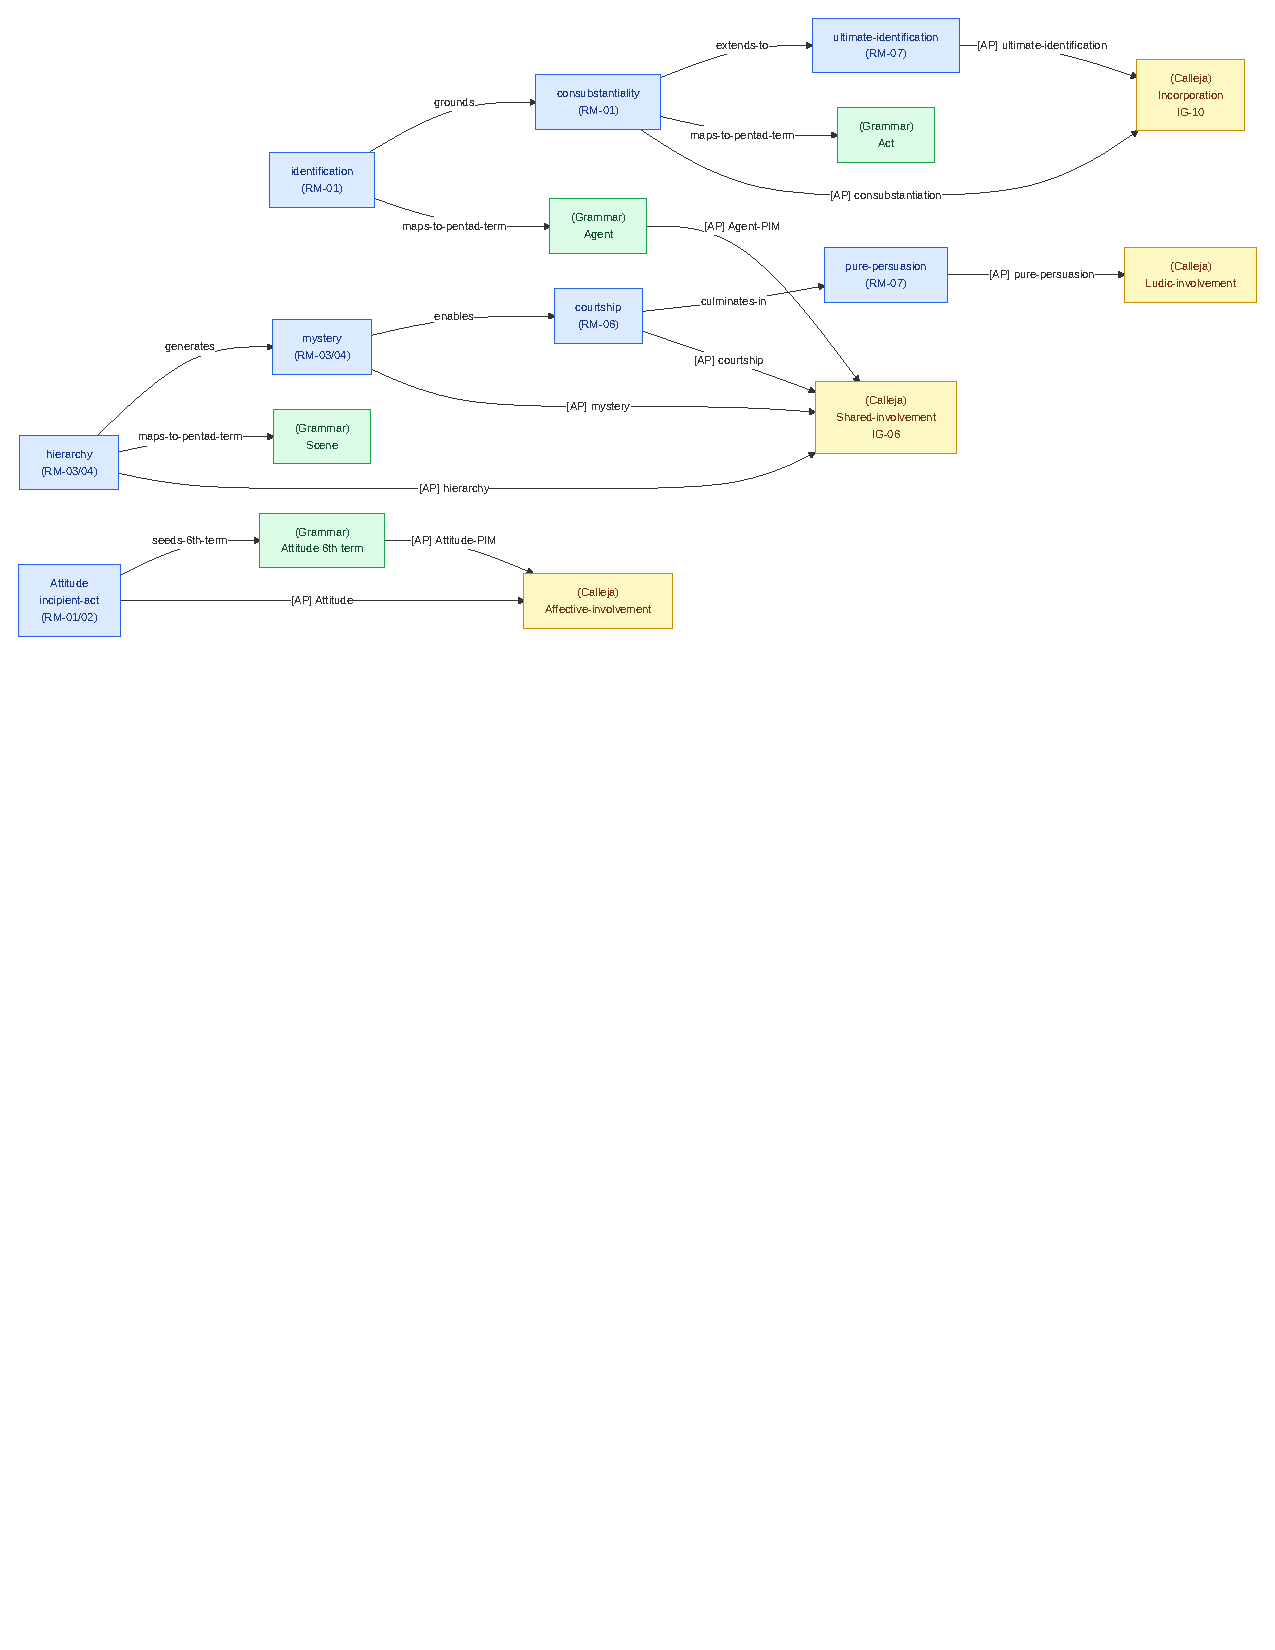
\includegraphics[width=\textwidth,height=0.82\textheight,keepaspectratio]{fig-bridge.pdf}
\caption{Burke (\textit{Rhetoric} $\times$ \textit{Grammar}) $\times$ Calleja PIM cross-pipeline bridge. Solid edges are \texttt{burke-direct}; edges marked [AP] are \texttt{anticipatory-projection}.}
\end{figure}
\end{document}
